%& -shell-escape
\documentclass[12pt]{article}
\usepackage[paperwidth=5.33in, paperheight=3.0in, top=0.35in, footskip=0.25in, bottom=0.25in, left=0.4in, right=0.4in]{geometry} %Sets Page Margins and landscape mode
\usepackage[usenames,dvipsnames]{xcolor}  %  Allows for named colors
\usepackage[ampersand]{easylist}  % Allows for nested lists
\usepackage{amsmath, amsthm, latexsym, amssymb}
\usepackage[shortlabels]{enumitem}%Allows styles in enumerate
\usepackage{amsfonts}
\usepackage{changepage}% allows adjust width
\usepackage[english]{babel}
\usepackage[latin1]{inputenc}
\usepackage{mathtools} % Allows coloneqq command
\usepackage{multicol}  %  Allows for mulitple columns
\usepackage{ulem}
\usepackage{cite} %Allows BibTex Citations
\usepackage{eso-pic}  %Used to set Slide Background Pictures
\usepackage[noindentafter,explicit]{titlesec}  %Formatsection Titles
\usepackage{fancyhdr}
\usepackage{lastpage}
\usepackage{pagecolor}  %changes color of page
\usepackage[colorlinks=true]{hyperref}  %hides boxes around hyperlinks
\usepackage[scaled]{helvet}
\renewcommand*\familydefault{\sfdefault} %% Only if the base font of the document is to be sans serif
\usepackage[T1]{fontenc}
\usepackage[EULERGREEK]{sansmath}  %Allows for capital greek letters in sansmath
\usepackage{wrapfig}


\sansmath
\usepackage{comment}
\usepackage{nameref}  %Allows Referencing The Slide Names
\usepackage{bm}
\usepackage{cancel}
\usepackage{setspace} %Adjust line spacing
\usepackage{overlays}
\usepackage{xcolor}

\usepackage{tikz}
\usepackage{pgfplots}
\usetikzlibrary{spy,backgrounds}
\usetikzlibrary{patterns}

\makeatletter
\newcommand{\pgfplotsdrawaxis}{\pgfplots@draw@axis}
\makeatother
\pgfplotsset{only axis on top/.style={axis on top=false, after end axis/.code={
             \pgfplotsset{axis line style=opaque, ticklabel style=opaque, tick style={thick,opaque},
                          grid=none}\pgfplotsdrawaxis}}}

\usepackage{boxedminipage}
\usepackage{listings}
\lstset{language=[LaTeX]TeX,breaklines=true}

\usepackage[outline]{contour}
\contourlength{1pt}

\definecolor{background}{HTML}{303030}
\definecolor{defaultcolor}{HTML}{DDDDDD}
\color{defaultcolor}

\fancyhf{}

\newcounter{IOlastslide}
\setcounter{IOlastslide}{1}
\newcommand{\lastslide}{\setcounter{IOlastslide}{0}}  %Use this command to indicate last slide
%Sets up page numbering
\setlength{\headheight}{0pt}
\rfoot{ \raisebox{10pt}{\tiny\bfseries \thepage /\pageref*{LastPage}\hspace{-0.125in}} \vfill} 
\renewcommand{\headrulewidth}{0pt}  

\newcommand{\Red}[1]{ {\color{DarkRed} #1} }
\newcommand{\Blue}[1]{ {\color{DarkBlue} #1} }

%%%%%%%%%%  Setting Up Equation Numbering / Creating Custom Environments %%%%%%%%%%
\renewcommand{\theequation}{\arabic{equation}}  %Changes Equation Numbering
\newcounter{oldequation}
\newcounter{definition}
\newenvironment{proof*}{{\noindent {\it Proof.  \ignorespaces}}}{\hfill$\blacksquare$}
\newenvironment{labeledproof}[1]{\noindent {\it Proof of {#1}}. \ignorespaces}{\hfill$\blacksquare$}
\newtheorem{theorem}{Theorem}
\newtheorem{lemma}[theorem]{Lemma}
\newtheorem{coro}[theorem]{Corollary}
\newtheoremstyle{example}% <name>
{3pt}% <Space above>
{3pt}% <Space below>
{}% <Body font>
{}% <Indent amount>
{\bfseries}% <Theorem head font>
{.}% <Punctuation after theorem head>
{0.5em}% <Space after theorem headi>
{}% <Theorem head spec (can be left empty, meaning `normal')>
\theoremstyle{example}
\newtheorem{example}{Example}[subsection]
\newtheoremstyle{defn}% <name>
{3pt}% <Space above>
{3pt}% <Space below>
{}% <Body font>
{}% <Indent amount>
{\bfseries}% <Theorem head font>
{.}% <Punctuation after theorem head>
{.5em}% <Space after theorem headi>
{}% <Theorem head spec (can be left empty, meaning `normal')>
\theoremstyle{defn}
\newtheorem{defn}[definition]{Definition}
\newtheorem{prop}[theorem]{Proposition}
\newtheorem{rmk}[theorem]{Remark}
%\newenvironment{rmk}{\noindent {\bfseries{Remark.\ }}}
%{\vspace{3pt}}
%%%%%%%%%%  Finished Setting Up Equation Numbering / Creating Custom Environments %%%%%%%%%%


%%%%%%%%%%  Setting Up Custom Commands %%%%%%%%%%
\newcommand{\K}{\operatornamewithlimits{K}}  %used to have \limits after {K} (continued fraction notation)
\newcommand{\genpocq}[3]{\left(q^{#1};q^{#2}\right)_{#3}}  %pochammer notation
\newcommand{\genpocaq}[3]{\left(#1;q^{#2}\right)_{#3}}  %pochammer notation
\newcommand{\kfrac}[2]{\frac{#1}{#2}\genfrac{}{}{0pt}{}{}{+}} %continued fraction notation
\newcommand{\lowfrac}[1]{\genfrac{}{}{0pt}{}{}{#1}}  %Makes a fraction without a bar with input in denominator
\newcommand{\dlowfrac}[1]{\genfrac{}{}{0pt}{}{\phantom{a_n}}{#1}} %As above but with at least a space for a_n in numerator.
\newcommand{\tcent}[1]{\hspace*{\fill} #1 \hspace*{\fill}}  %Used horizontally center entries in a table
\renewcommand{\emph}{\textit}
\renewcommand{\bmod}{\operatorname{mod} \, }
\renewcommand{\vec}{\mathbf} %{\boldsymbol}  %changes vectors to bold face

\usetikzlibrary{pgfplots.statistics, pgfplots.colorbrewer} 
% provides \pgfplotstabletranspose
\usepackage{pgfplotstable}
\usepackage{filecontents}

\makeatletter
\pgfplotsset{
    boxplot prepared from table/.code={
        \def\tikz@plot@handler{\pgfplotsplothandlerboxplotprepared}%
        \pgfplotsset{
            /pgfplots/boxplot prepared from table/.cd,
            #1,
        }
    },
    /pgfplots/boxplot prepared from table/.cd,
        table/.code={\pgfplotstablecopy{#1}\to\boxplot@datatable},
        row/.initial=0,
        make style readable from table/.style={
            #1/.code={
                \pgfplotstablegetelem{\pgfkeysvalueof{/pgfplots/boxplot prepared from table/row}}{##1}\of\boxplot@datatable
                \pgfplotsset{boxplot/#1/.expand once={\pgfplotsretval}}
            }
        },
        make style readable from table=lower whisker,
        make style readable from table=upper whisker,
        make style readable from table=lower quartile,
        make style readable from table=upper quartile,
        make style readable from table=median,
        make style readable from table=lower notch,
        make style readable from table=upper notch
}
\makeatother

\usepackage{minted}
\usepackage{xcolor}
\definecolor{LightGray}{gray}{0.90}
\usepackage[explicit]{titlesec}
\usepackage{amsmath}
\usepackage{nameref}
\usepackage[colorlinks=true]{hyperref}
\usepackage{textcomp} %For adding < >
\usepackage{graphicx}
\usepackage{listings}
\usepackage{mdframed}

\titleformat{\section}{\normalfont\Large\bfseries}{}{0em}{#1} %add this after #1 to include section number\ \thesection}


\newminted[pythoncode]{python}{frame=lines,framesep=2mm,baselinestretch=1.2,bgcolor=Black,fontsize=\footnotesize,linenos}
\newminted[sqlcode]{sql}{frame=lines,framesep=2mm,baselinestretch=1.2,bgcolor=Black,fontsize=\footnotesize,linenos}
\newminted[httpcode]{html}{frame=lines,framesep=2mm,baselinestretch=1.2,bgcolor=Black,fontsize=\footnotesize,linenos}

\newcommand{\mintedpython}[1]{\inputminted[frame=lines,framesep=2mm,baselinestretch=1.2,bgcolor=Black,fontsize=\footnotesize,linenos]{python}{#1}}
\newcommand{\mintedsql}[1]{\inputminted[frame=lines,framesep=2mm,baselinestretch=1.2,bgcolor=Black,fontsize=\footnotesize,linenos]{sql}{#1}}
\newcommand{\mintedhttp}[1]{\inputminted[frame=lines,framesep=2mm,baselinestretch=1.2,bgcolor=Black,fontsize=\footnotesize,linenos]{html}{#1}}

\begin{document}






\pagestyle{fancy}
\setlength{\parindent}{0pt}
\setlength{\parskip}{12pt}
\setlength{\columnsep}{0.4in}
\thispagestyle{empty} %Gets Rid of Page Number
\pagecolor{background}
\setcounter{page}{0}

\vspace*{\fill}




\setcounter{section}{14}
\setcounter{subsection}{3}

\setcounter{example}{0}

\vspace*{\fill}

\begin{center}
\begin{spacing}{1.5}
\begin{Large}
Media bias
\end{Large}
\end{spacing}


\vspace*{12pt}
{Michael Kuhn

Herman Schaumburg

May 9, 2020}


\end{center}

\vspace*{\fill}

\clearpage


{Goals}

\vspace*{-16pt}
\begin{footnotesize}
\begin{itemize}[\label{}]
\item Primary: Find objective way to score bias in 36 selected news organizations.
\item Secondary: Estimate the political bias of a given tweet.
\item Secondary: Heroku deployment.
\end{itemize}
\end{footnotesize}

\clearpage

\vfill

\hspace*{\fill}
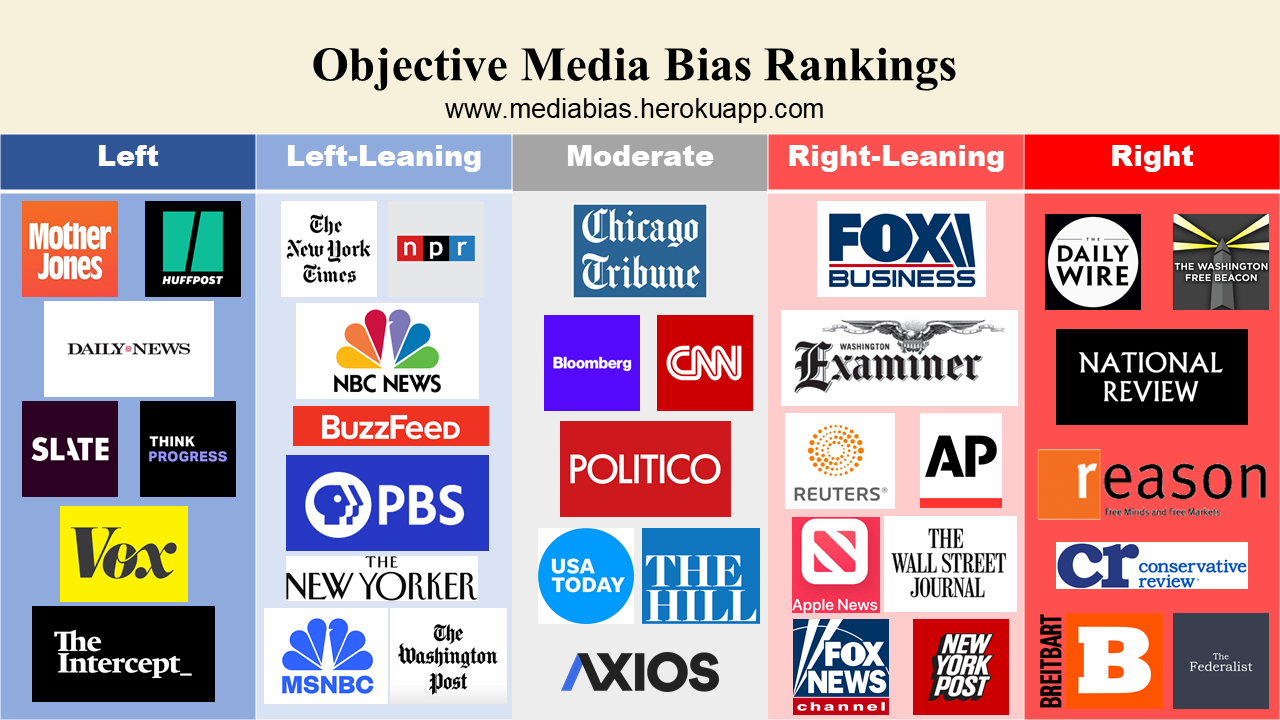
\includegraphics[scale=0.3]{mediabiaschart.png}
\hspace*{\fill}

\vspace*{\fill}

\vfill

\clearpage

{\large DW-NOMINATE scores}

\vspace*{-5pt}
\hspace*{\fill}
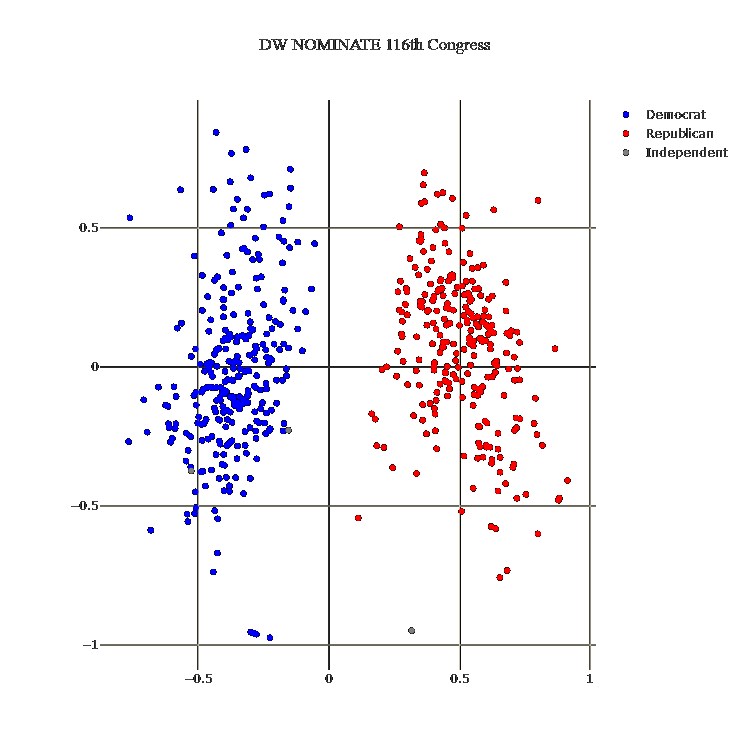
\includegraphics[scale=0.2]{dwnominate_pic_white.png}
\hspace*{\fill}

\clearpage

{\large Methodology}

\vspace*{-16pt}
\begin{enumerate}
\item Gathered tweets from Democratic and Republican law makers (1,266,104) from Alex Litel github repository into SQL database.  From media orgs 54,833.

https://github.com/alexlitel/congresstweets

\item DW-NOMINATE scores of congress people from voteview

https://voteview.com/data
\item Queried tweets of congresspeople for the media domains they tweet from and used the congressperson DW-NOMINATE score to score the media domain.
\end{enumerate}



\clearpage

{\large Media domain scores}

\vspace*{-5pt}
\hspace*{\fill}
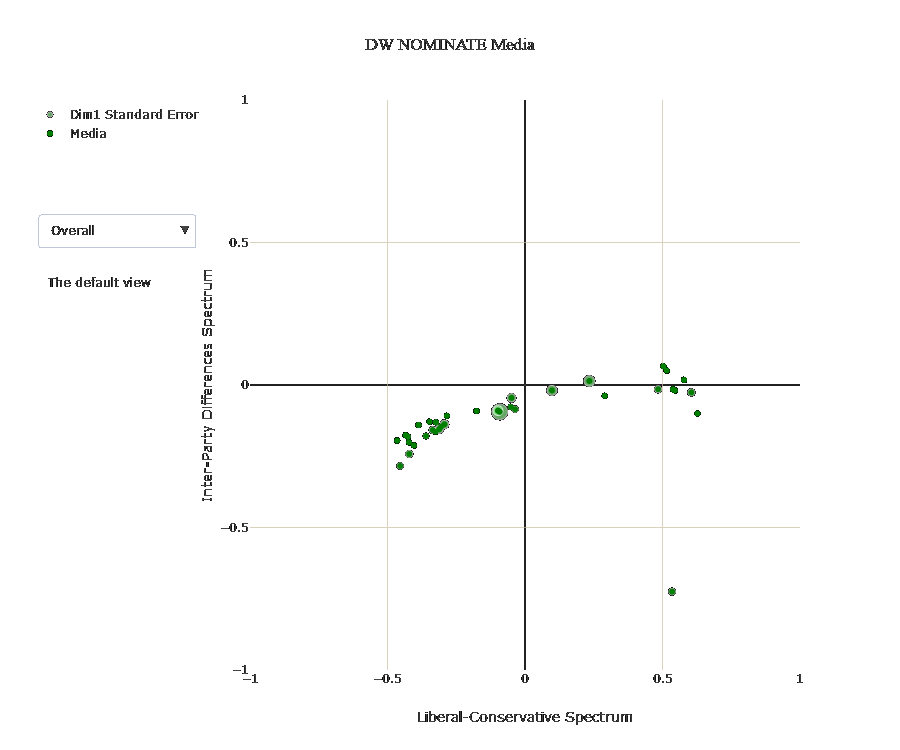
\includegraphics[scale=0.2]{media_pic_white.png}
\hspace*{\fill}

\clearpage

Method diagram

\vspace*{-10pt}
\hspace*{\fill}
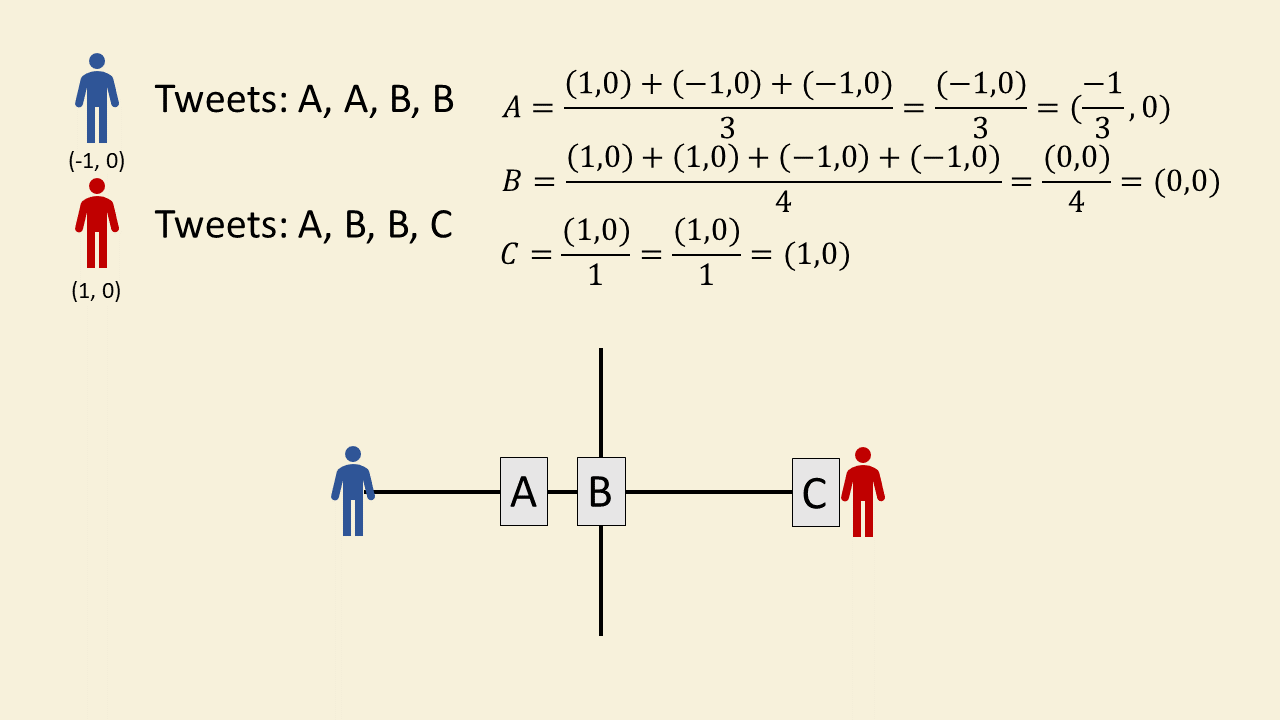
\includegraphics[scale=0.25]{method_visual2.png}
\hspace*{\fill}

\clearpage

Bias Ranking

\hspace*{\fill}
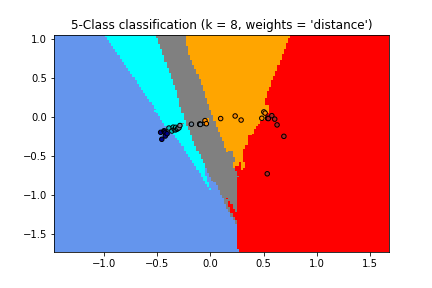
\includegraphics[scale=0.4]{5class.png}
\hspace*{\fill}

\vspace*{-10pt}
{\small
K-Nearest neighbors to classify media domains: 

\vspace*{-10pt}
\hspace*{\fill}Left, Left-leaning, Moderate, Right-leaning, Right
}

\clearpage


SQL Schema

\hspace*{\fill}
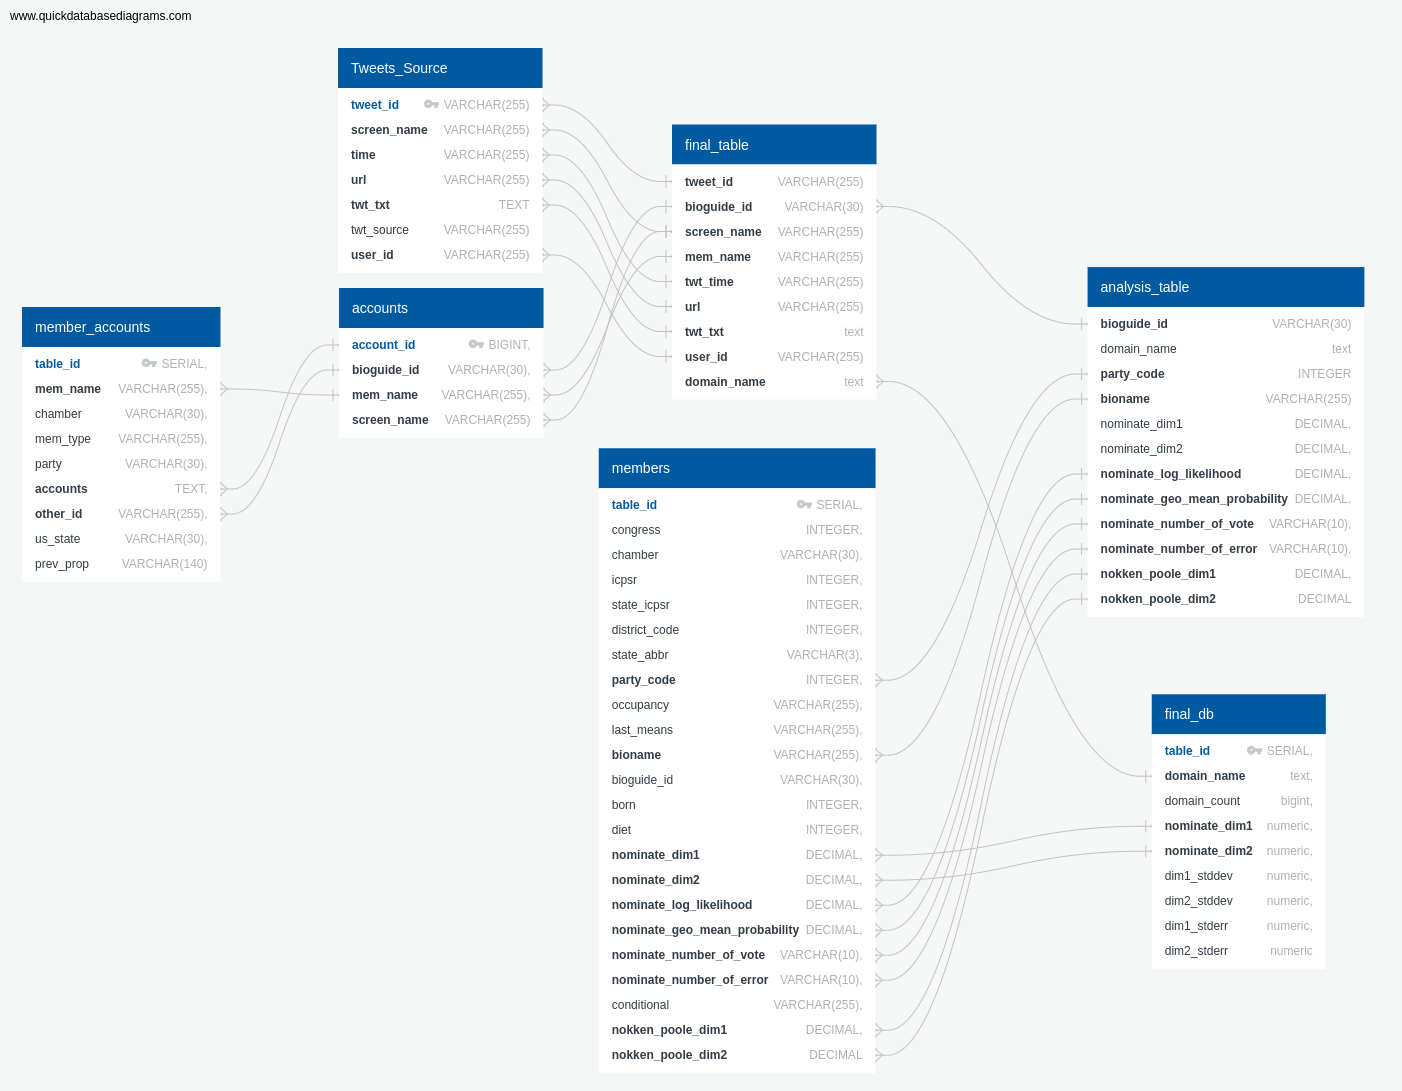
\includegraphics[scale=0.13]{QuickDBD-Media_Bias_DB.png}
\hspace*{\fill}

\clearpage

ML Model Selection

\hspace*{\fill}
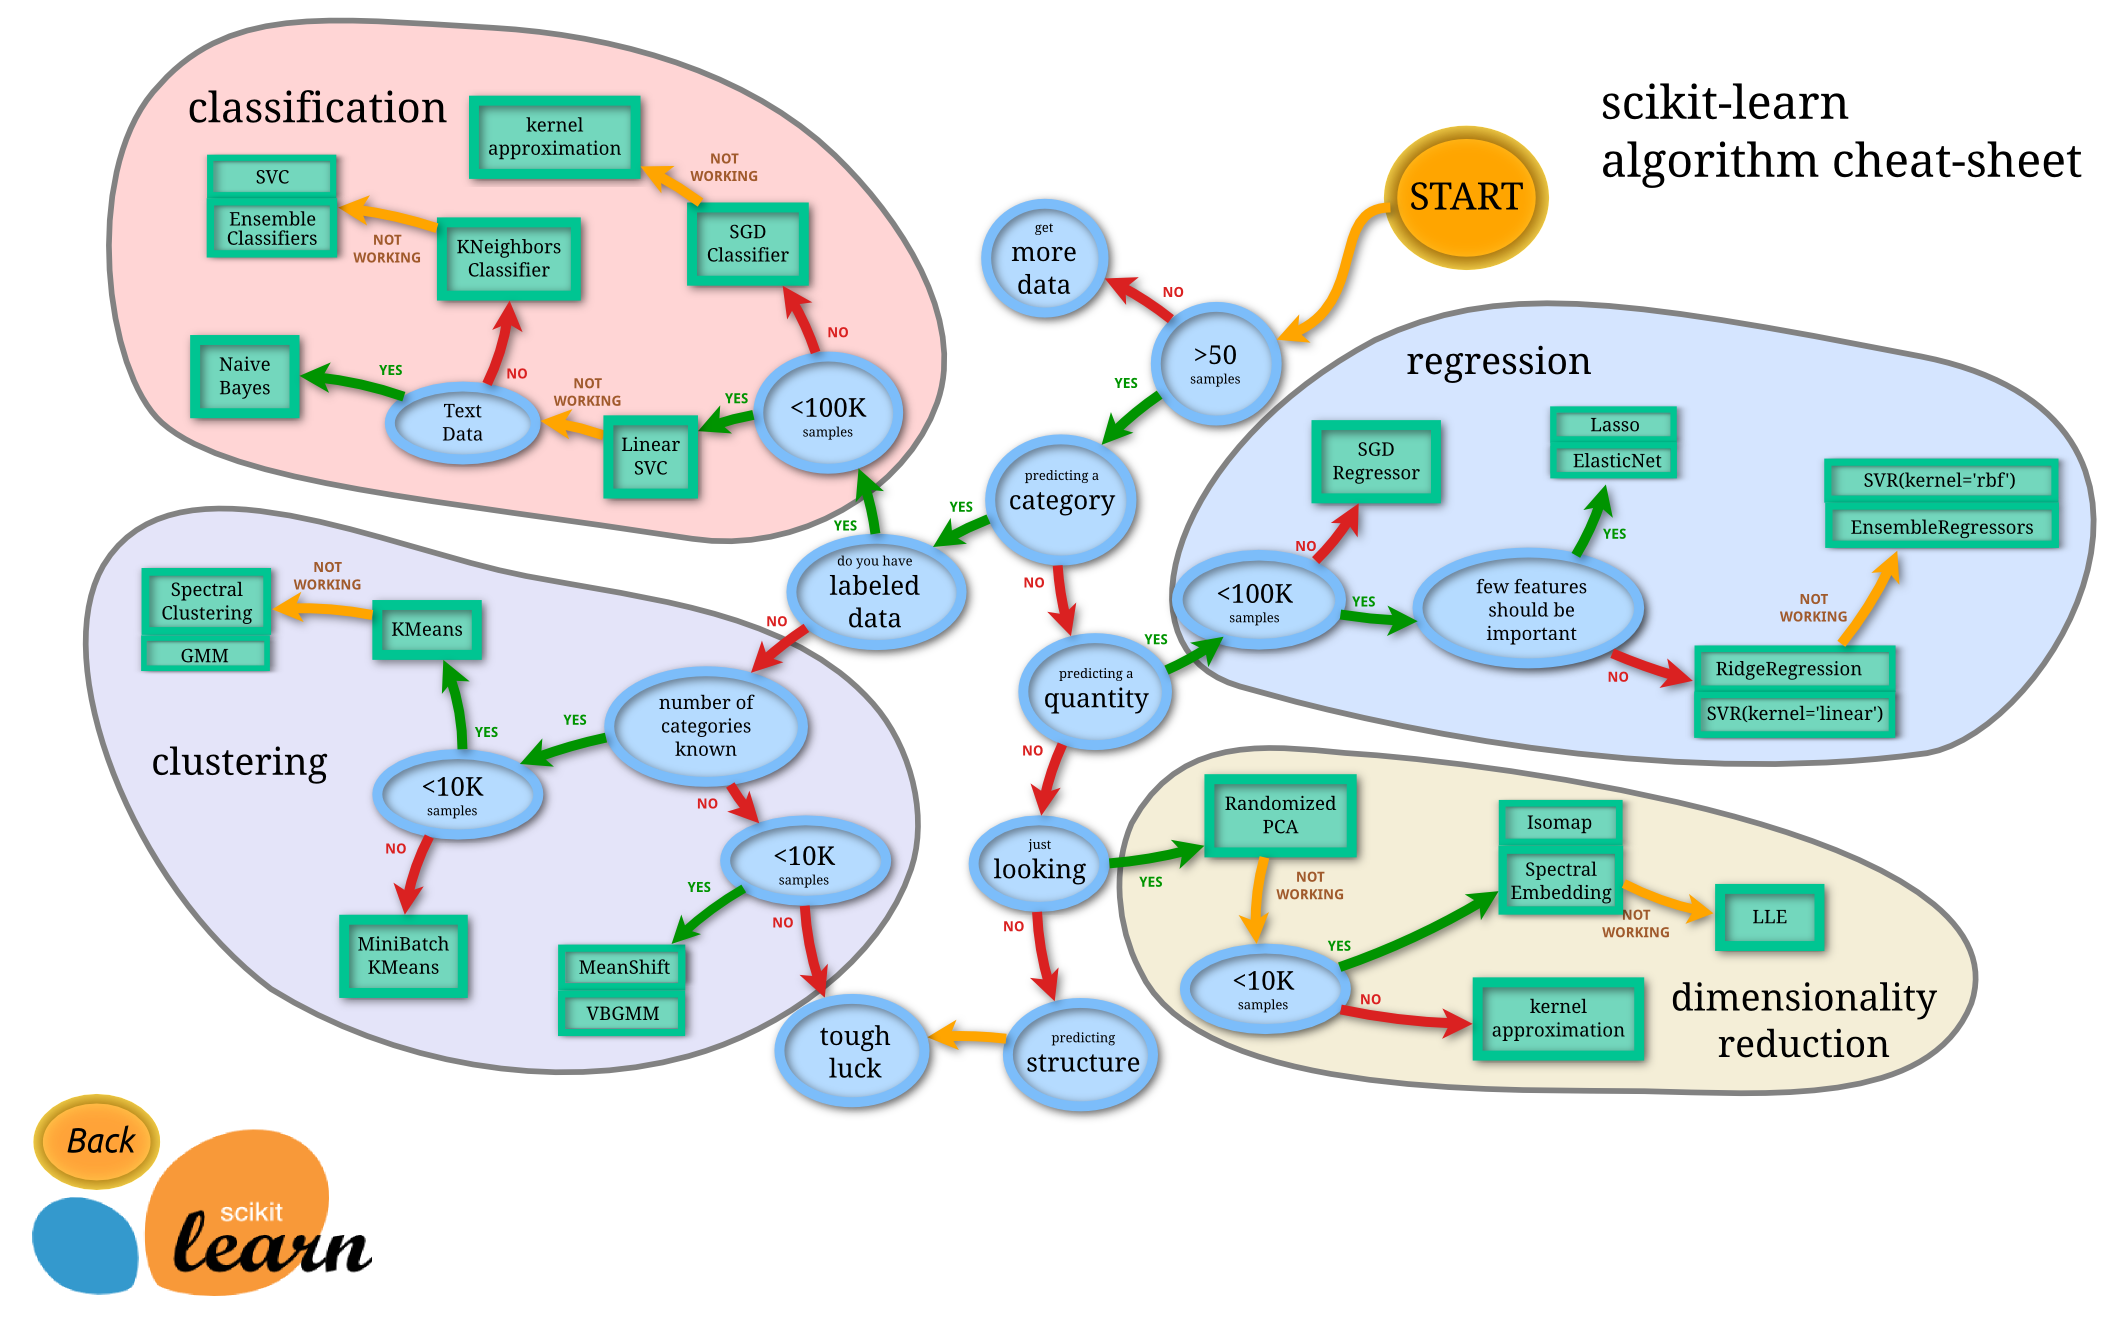
\includegraphics[scale=0.06]{ml_map.png}
\hspace*{\fill}

\clearpage

ML Model

\vspace*{-10pt}
\begin{enumerate}
\item Use nltk to remove stopwords from tweets.
\item Tweets are vectorized using several schemes (used {\textasciitilde}15K tweets).
\item Best performing scheme is selected for fine tuning.
\item End result is Stochastic Gradient Decent Model with 0.8482 score on large selection of tweets ({\textasciitilde}64K tweets).
\item Empirical CDF of errors in large test used to estimate probability of making an error.
\end{enumerate}

\clearpage

Vectorized Tweets

\begin{tiny}
\begin{verbatim}
  (0, 599005)	0.13724572483536815
  (0, 598951)	0.10656565688654346
  (0, 597099)	0.07127021892848737
  (0, 596894)	0.0696688776808445
  (0, 596846)	0.0835728977646812
  (0, 596744)	0.07270567427770662
  (0, 581647)	0.08857473689547032
  (0, 581646)	0.08857473689547032
  (0, 568348)	0.21930758305074324
  (0, 568331)	0.1444337225102922
  (0, 548752)	0.08863406696726873
\end{verbatim}
\end{tiny}

\clearpage

Test for normality failed - p-value near zero (couldn't use prediction interval)

\hspace*{\fill}
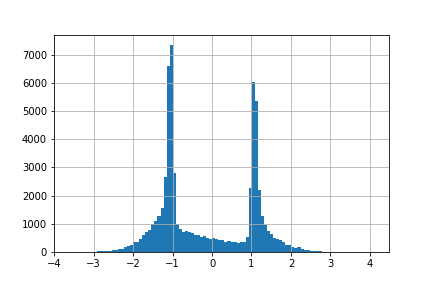
\includegraphics[scale=0.45]{histogram.png}
\hspace*{\fill}

\clearpage


Empirical Complementary CDF

\hspace*{\fill}
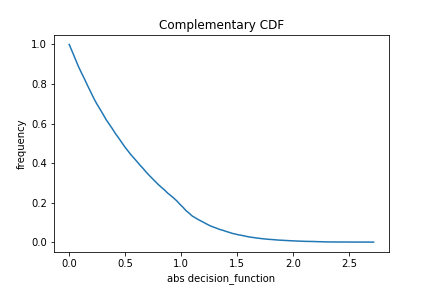
\includegraphics[scale=0.45]{complementary_cdf.png}
\hspace*{\fill}

\clearpage

\hspace*{\fill}

{\large Passing user input to flask app}

\hspace*{\fill}
\scalebox{0.6}{
\begin{minipage}{1.6\textwidth}
%\definecolor{bg}{rgb}{0,0,0}
%\begin{mdframed}[backgroundcolor=bg]
\mintedhttp{html_snippet.html}
%\end{mdframed}
\end{minipage}
}
\hspace*{\fill}

\clearpage


Second model attempted

Attempted to use Stochastic Gradient Decent Regression Model to get dw nominate score of tweeter.

Training $R^2 = 0.95$ and test $R^2 =0.5$.

\clearpage


{\large Heroku deployment features}

\begin{itemize}
\item About page - interactive plots.
\item ML models page - text box to predict party of tweeter.
\item Search Media Scores Page - text box to search SQL data base for media domain.
\end{itemize}

\clearpage

{\large Heroku difficulty}

Flask app, \texttt{app.py}, is in a separate directory from heroku config files. This made it difficult to load the scikit learn models into the app.  The issue was resolved using by printing information to the page on the current working directory using the os library if the models failed to run:


\hspace*{\fill}
\scalebox{0.6}{
\begin{minipage}{1.6\textwidth}{
\mintedpython{heroku_trouble.py}
}
\end{minipage}
}
\hspace*{\fill}

\clearpage

SQL Query

\hspace*{\fill}
\scalebox{0.65}{
\begin{minipage}{1.5\textwidth}
\mintedsql{sql_query.sql}
\end{minipage}
}
\hspace*{\fill}

\clearpage



jsonToCSV

\hspace*{\fill}
\scalebox{0.42}{
\begin{minipage}{1.25\textwidth}{
\mintedpython{csv2json.py}
}
\end{minipage}
}
\hspace*{\fill}

\clearpage



\end{document}


(r,15) 
(t,11) 
(a,10) 
(o,10) 
(i,9) 
%(s,9) 
(c,8) 
(m,6) 
%(l,6) 
%(n,6) 
(u,5) 
(h,5) 
%(d,4) 
(f,4) 
%(w,3) 
%(b,2) 
%(p,2) 
(y,2) 
%(S,1) 
%(z,1) 
(v,1) 
%(U,1) 
%(g,1)};  
\end{axis}  
